\section{State of the Art}

\subsection{Traditional Soundscape Generation}

\begin{frame}
    \frametitle{Traditional Soundscape Generation}

    \textbf{Notable Tools}
    \begin{itemize}
        \item \textit{Scaper}~\cite{salamon_scaper_2017}: Open-source library for synthetic sound environments
        \item SEED~\cite{bernardes_seed_2016}: System for resynthesizing environmental sounds with precise control over variation
        \item Physics-Based Concatenative Sound Synthesis~\cite{magalhaes_physics-based_2020}: Creates novel auditory experiences by assembling pre-existing sound segments
    \end{itemize}
\end{frame}

\subsection{Unsupervised Sound Generation}

\begin{frame}
    \frametitle{Unsupervised Sound Generation}

    \textbf{Approach}
    \begin{itemize}
        \item Learn sound features and distributions without explicit labels
        \item Utilize unlabeled audio data for pattern capture and structure learning
        \item Valuable when labeled datasets are limited or costly
    \end{itemize}

    \textbf{Notable Models}
    \begin{itemize}
        \item WaveGAN~\cite{donahue_adversarial_2019}: Unsupervised waveform synthesis using modified GAN
        \item Generative Transformer~\cite{verma_generative_2021}: Autoregressive prediction of audio samples using transformer networks
        \item wav2vec 2.0~\cite{baevski_wav2vec_2020}: Speech generation model with convolutional feature encoder, Transformer, and quantization module
        \item SoundStream~\cite{zeghidour_soundstream_2021}: Neural audio codec for efficient audio compression
    \end{itemize}
\end{frame}


\subsection{Vocoders}

\begin{frame}
    \frametitle{Vocoders}

    \textbf{Notable Models}
    \begin{itemize}
        \item WaveNet~\cite{oord_wavenet_2016}: Generative neural network using dilated causal convolutions for raw audio waveform generation
        \item WaveNet Variants: Models like WaveRNN, FloWaveNet, and Fast WaveNet reduce complexity while maintaining effectiveness
        \item MelGAN~\cite{kumar_melgan_2019}: GAN-based model using Mel-Spectrograms for coherent audio waveform generation
        \item GANSynth~\cite{engel_gansynth_2019}: GAN using log-magnitude spectrograms and phases for waveform generation
        \item HiFi-GAN~\cite{kong_hifi-gan_2020}: GAN model combining efficiency and high-fidelity speech synthesis
    \end{itemize}
\end{frame}


\subsection{End-to-End Models}


\begin{frame}
    \frametitle{End-to-End Audio Models Comparison}

    \begin{table}[ht]
        \centering
        \caption{A comparison of different end-to-end generative models for audio.}
        \begin{tabularx}{\textwidth}{|X|l|X|X|}
            \hline
            \textbf{Model}                           & \textbf{Type} & \textbf{Input}            & \textbf{Output}    \\ \hline
            Char2wav~\cite{sotelo_char2wav_2017}     & Speech        & Text prompt               & Raw audio waveform \\ \hline
            VALL-E~\cite{wang_neural_2023}           & Speech        & Text and acoustic prompt  & Raw audio waveform \\ \hline
            Jukebox~\cite{dhariwal_jukebox_2020}     & Music         & Genre, artist, and lyrics & Raw audio waveform \\ \hline
            Riffusion~\cite{forsgren_riffusion_2022} & Music         & Text prompt               & Raw audio waveform \\ \hline
            MusicLM~\cite{agostinelli_musiclm_2023}  & Music         & Text prompt               & Raw audio waveform \\ \hline
            SampleRNN~\cite{mehri_samplernn_2017}    & General       & None                      & Raw audio waveform \\ \hline
        \end{tabularx}
        \label{tab:end-to-end-audio-models}
    \end{table}
\end{frame}

\begin{frame}
    \frametitle{End-to-End Audio Models Comparison (Cont.))}

    \begin{table}[ht]
        \centering
        \caption{A comparison of different end-to-end generative models for audio.}
        \begin{tabularx}{\textwidth}{|X|l|X|X|}
            \hline
            \textbf{Model}                       & \textbf{Type} & \textbf{Input} & \textbf{Output}                        \\ \hline
            AudioLM~\cite{borsos_audiolm_2022}   & General       & Text prompt    & Raw audio waveform                     \\ \hline
            DiffSound~\cite{yang_diffsound_2022} & General       & Text prompt    & Mel-spectrogram and raw audio waveform \\ \hline
            AudioGen~\cite{kreuk_audiogen_2023}  & General       & Text prompt    & Mel-spectrogram and raw audio waveform \\ \hline
        \end{tabularx}
    \end{table}
\end{frame}

\begin{frame}
    \frametitle{Text-to-Speech (TTS)}

    \textbf{Definition}
    \begin{itemize}
        \item Convert written text into synthesized speech
        \item Use deep neural networks for direct mapping
        \item Notable TTS Models:
              \begin{itemize}
                  \item Char2wav
                  \item VALL-E
              \end{itemize}
    \end{itemize}
\end{frame}

\begin{frame}
    \frametitle{Generative Music}

    \textbf{Definition}
    \begin{itemize}
        \item Create music using generative techniques
        \item End-to-end models for composing new musical pieces
        \item Notable Generative Music Models:
              \begin{itemize}
                  \item Jukebox
                  \item Riffusion
                  \item MusicLM
              \end{itemize}
    \end{itemize}

\end{frame}

\begin{frame}
    \frametitle{General Text-to-Audio}

    \textbf{Definition}
    \begin{itemize}
        \item Convert various forms of text to corresponding audio outputs
        \item Applications: sound effects, voice transformation, environmental sound synthesis
        \item Notable Text-to-Audio Models:
              \begin{itemize}
                  \item SampleRNN
                  \item AudioLM
                  \item DiffSound
                  \item AudioGen
              \end{itemize}
    \end{itemize}

\end{frame}


\subsection{AudioLM}
\begin{frame}{AudioLM}

    \begin{figure}
        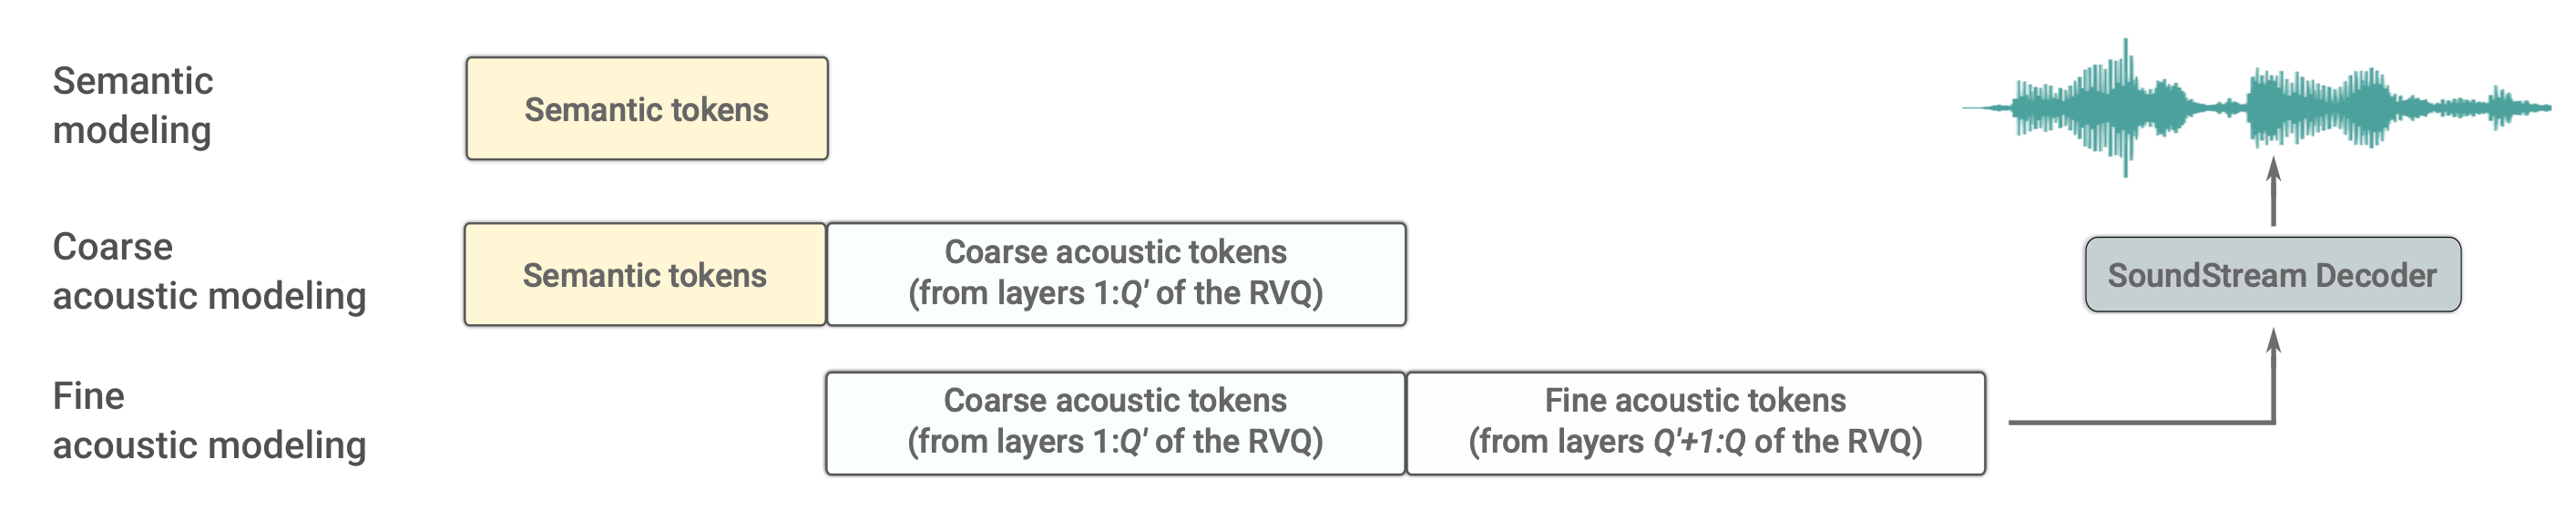
\includegraphics[width=\textwidth]{images/2-sota/audiolm.png}
        \caption{Illustration of the AudioLM model architecture \cite{borsos_audiolm_2022}.}
        \label{fig:audiolm}
    \end{figure}

    \note{
        \begin{itemize}
            \item A framework for high-quality audio generation with long-term consistency~\cite{borsos_audiolm_2022}.
            \item Maps input audio to a sequence of discrete tokens and treats audio generation as a language modeling task.
            \item Achieves high-quality synthesis and long-term structure through a hybrid tokenization scheme of semantic and acoustic tokens.
            \item Consists of three main components: tokenizer, language model, and detokenizer.
            \item Generates syntactically and semantically plausible speech and music continuations without any transcript or annotation.
        \end{itemize}
    }
\end{frame}

\subsection{DiffSound}

\begin{frame}{DiffSound}

    \begin{figure}
        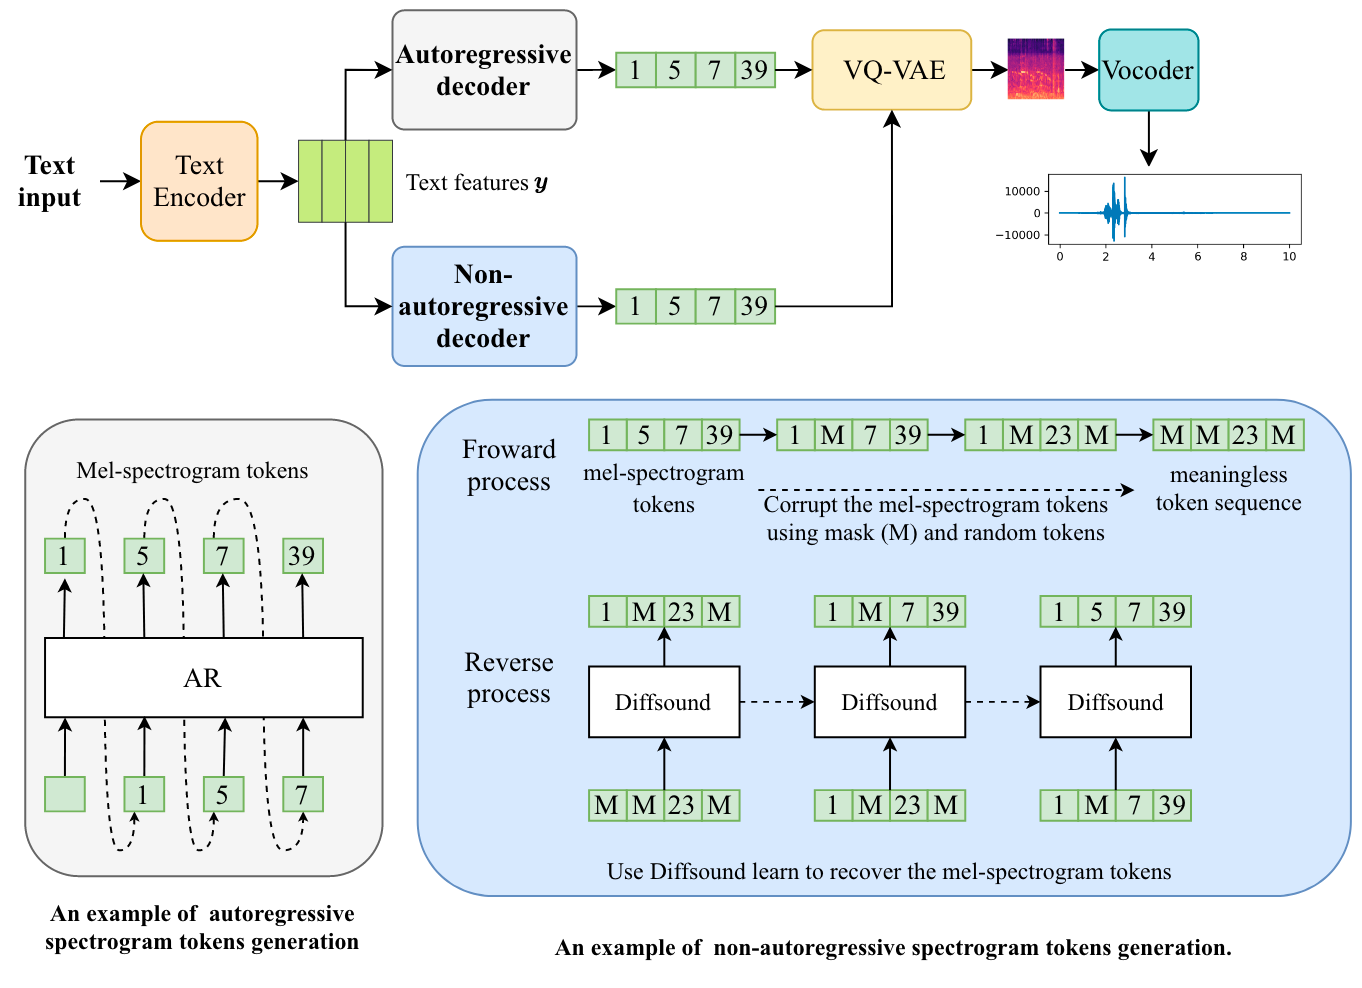
\includegraphics[width=\textwidth, height=0.7\textheight, keepaspectratio]{images/2-sota/diffsound.png}
        \caption{Illustration of the DiffSound model architecture \cite{yang_diffsound_2022}.}
        \label{fig:diffsound}
    \end{figure}

    \note{
        \begin{itemize}
            \item A novel text-to-sound generation framework that uses a text encoder, a VQ-VAE, a decoder, and a vocoder~\cite{yang_diffsound_2022}.
            \item Takes text as input and outputs synthesized audio corresponding to the input text.
            \item Uses a diffusion decoder (DiffSound) that predicts and refines all Mel-Spectrogram tokens in one step, resulting in better and faster generation than an AR decoder.
            \item Produces high-quality sound synthesis for various domains such as speech, music, and environmental sounds.
        \end{itemize}
    }
\end{frame}


\subsection{AudioGen}
\begin{frame}{AudioGen}

    \begin{figure}
        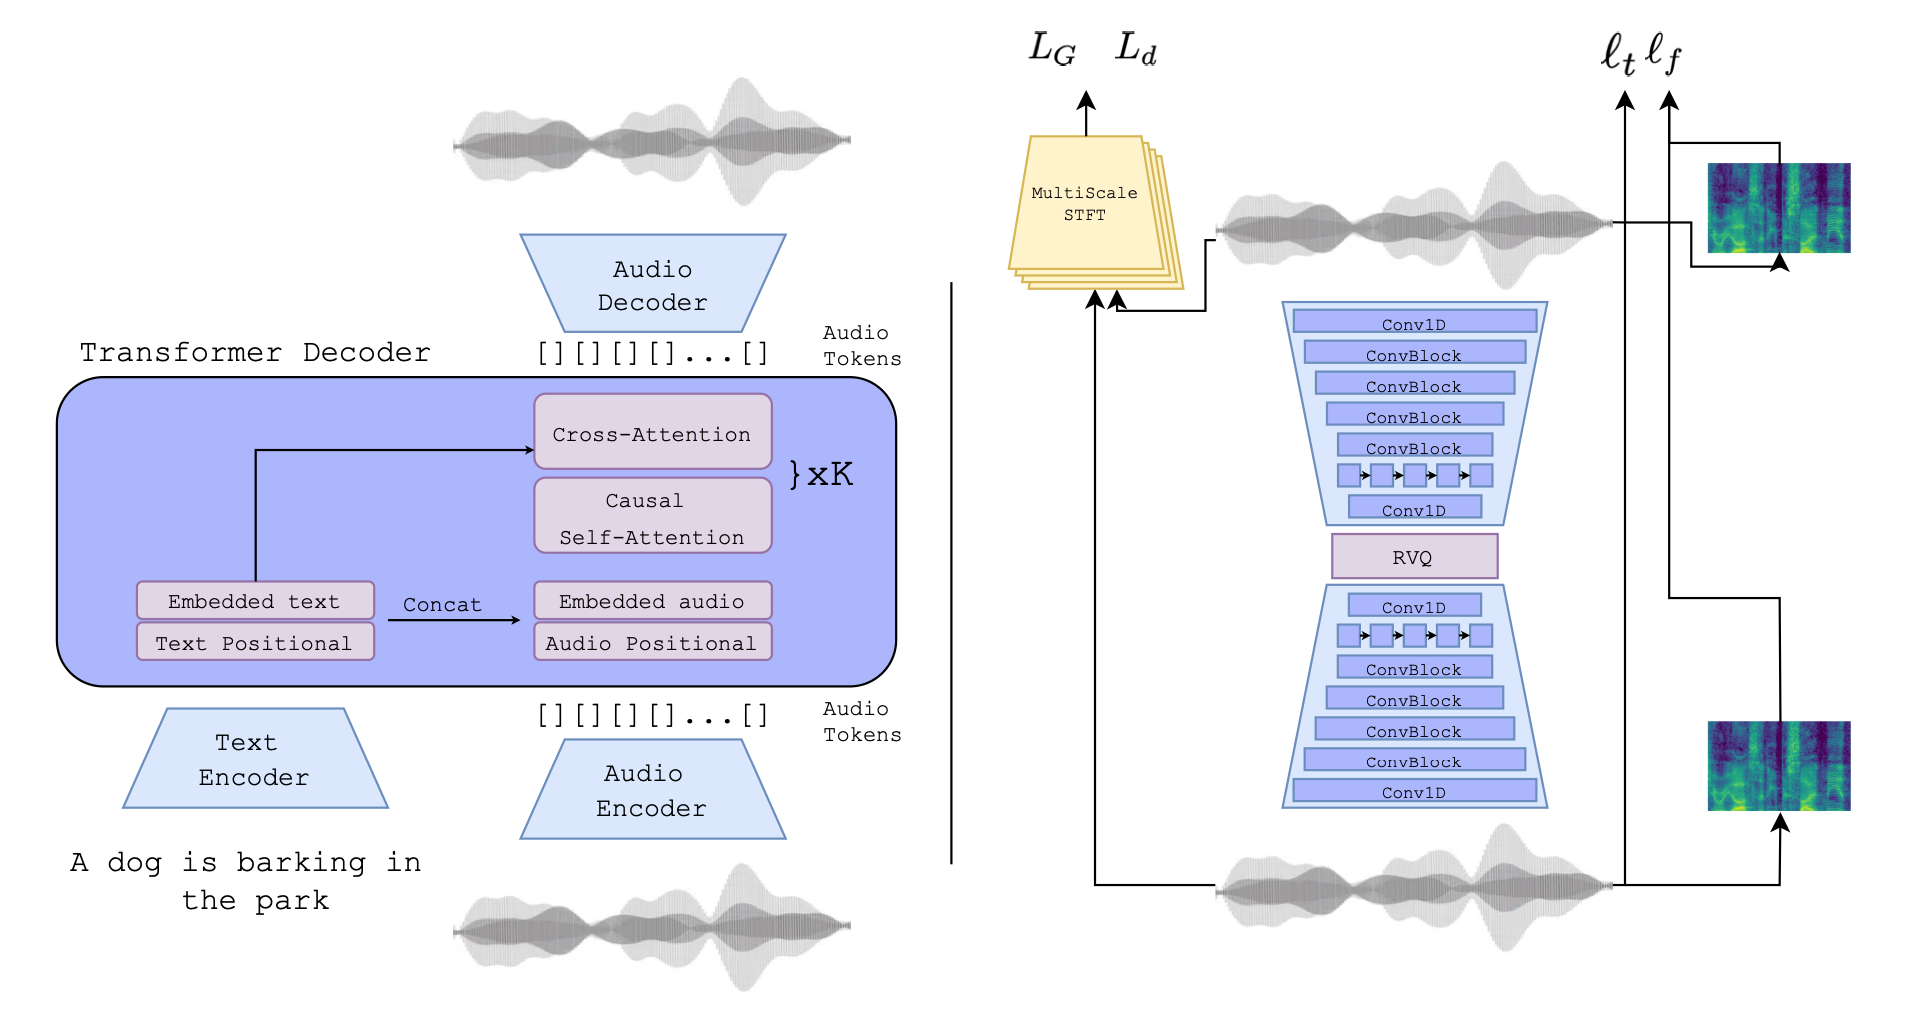
\includegraphics[width=\textwidth, height=0.7\textheight, keepaspectratio]{images/2-sota/audiogen.png}
        \caption{Illustration of the AudioGen model architecture \cite{kreuk_audiogen_2023}.}
        \label{fig:audiogen}
    \end{figure}

    \note{
        \begin{itemize}
            \item An auto-regressive generative model that generates audio samples conditioned on text inputs~\cite{kreuk_audiogen_2023}.
            \item Learns a discrete representation of the raw audio using an AE method and trains a Transformer language model over the learned codes, conditioned on textual features.
            \item Uses an augmentation technique that mixes different audio samples to train the model to separate multiple sources internally.
            \item Explores the use of multi-stream modeling for faster inference, allowing the use of shorter sequences while maintaining a similar bitrate and perceptual quality.
            \item Outperforms evaluated baselines over both objective and subjective metrics and extends to conditional and unconditional audio continuation.
        \end{itemize}
    }
\end{frame}
